\section{Discussion}

\subsection{Reduction}
As it as been mentioned in the introduction, the "abstraction reduction" does not always create smaller abstractions.
This depends on the type of inputs (discrete, continuous), the number of dimension of inputs, the dimension of the suppressed subspace of the state space and the initial discretization of it.

\subsection{Covering/Overlap in the state space}
When we replace the knowledge of part of the state by the estimation of the state based on inputs, there can be no equivalent discretization of the state space.
Mainly because 2 input sequences can produce reached sets that overlaps.
These overlap (see \ref{fig:overlapp}) cannot happened in discretization of the state space without any memory (the state is supposed to belong to one and only one observation).

We will see later that it can bring to improvement of the size of the abstraction in practice.

\begin{figure}
\centering
\begin{subfigure}[b]{0.49\textwidth}
	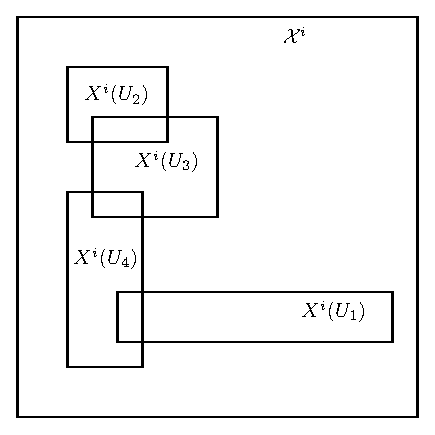
\includegraphics[width=\textwidth]{chapters/abstraction_reduction/overlapp_disc.eps}
\end{subfigure}	
\begin{subfigure}[b]{0.49\textwidth}
	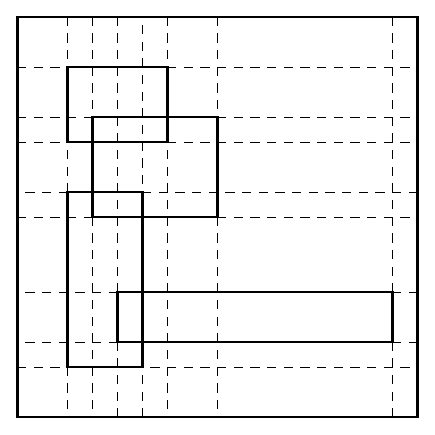
\includegraphics[width=\textwidth]{chapters/abstraction_reduction/overlapp_disc2.eps}
\end{subfigure}	
\caption{For the abstraction on the right, the reached sets overlapps. The equivalent discretization of the state space on the left create an abstraction of 72 symbols.}
\end{figure}

Dynamic of the successor volume.

Self loops -not cool for multi agent task, lose the time information.
Abstractions of asymptotically stable system present a disadvantage on the multiagent control side, for some controls, if the state does not evolve any more, the abstraction will take self loops.
In term multi agent control this make the problem more complex as the control generation: self loops tend to create systems that are asynchronous with all the problems that might occurs because of this (basically one of the agent might be be stopped).

size of invariants in the 

%TODO GRAPH TO SHOW IT (I can also do it for the second integrator)

We will see that in some case it produce way smaller abstraction.

\subsection{Error sensitivity}
As we do not observe $\xunobs$, the reduced abstraction is not sensible to the measurement error on $\xunobs$. More over, as $\xunobs$ does not have a direct impact on the measurement, the error on $\xunobs$ impact the observation as a cumulative error.

During the reduction of the abstraction process, the admissible noise magnitude remain the same. However, the constraints are different as the error does not have any more a direct impact on the state but can be propagating.
In this part, we will try to establish what are the new constraints that does apply on the noise.

If there is no closed form solution to it, do it for a stupid system or for the quad.

\subsection{Dynamic consideration of the unobserved system}
This method is really restrictive, it suppose that part of the system is already controlled and that the controlled part behave the same independently of the rest of the other states. In the case of dynamical systems, the dynamic is most of the time independent of the position. 
The monotone property used for the first system is a strong assumption as well. It is used in order to reduce the study to a finite number of points.

Over approximation of the set, so we will create always more successors -> That is why we should not apply this methods for slow dynamic. Useful to take in account the transient states if the sampling time is close to the sampling rate of the system.

Effect of $\Ninputs$ over the $V_w$: the size of $V_w$ will decrease at the same speed than the dynamic. To make it easy, we will consider the trajectory of the point starting from $\overline{\mathbf{x}}_c$ with a a noise set that is symmetric ($\mathcal{W} = \left [ -\overline{\mathbf{w}},\overline{\mathbf{w}} \right ]$). We want to compute the size of the box which contains all the possible states after $\Ninputs$ timesteps of the reduced system.
\begin{equation}
\begin{split}
{\mathbf{x}^r}_{\Ninputs} &= \overline{\mathbf{x}}^r A_r^{\Ninputs} + \overline{\mathbf{x}}^{r \infty}\\
\overline{\mathbf{x}}^{r \infty} &= (I-A_r)^{-1}\overline{\mathbf{w}}
\end{split}
\end{equation}

The volume of ${V_w}_{\Ninputs}$ is equal to the product of the different components of ${\mathbf{x}_c}_{\Ninputs}$.
\begin{equation}
{V_w}_{\Ninputs} = 2 \prod_{i=1}^n
{\mathbf{x}_c}_{\Ninputs}^i
\end{equation}

Therefore, it worth to use this technique with $\Ninputs>1$ if some dynamic of the system are the same timing constant than the sampling time (which make sense as we have supposed that reduced system is stable, so in a way it is controlled and most often we will try to control the slower dynamic with this abstraction techniques). When all the time constants are either much smaller or much faster, then $\Ninputs = 1$ is a good value.
This is not efficient neither if the noise of the model is too high (ie if the $\overline{\mathbf{x}}_c^{\infty}$ is close to the initial value $\overline{\mathbf{x}}_c$). See the figure \ref{reduced_system_bounds} that present these result on the quadruple tank process.

\begin{figure}[!ht]
 %Experiment made on the quadruple tank process with values taken in the article of Johanson with 		T1,T2,T3,T4 = (63.,91.,5.,56.)
  \centering
  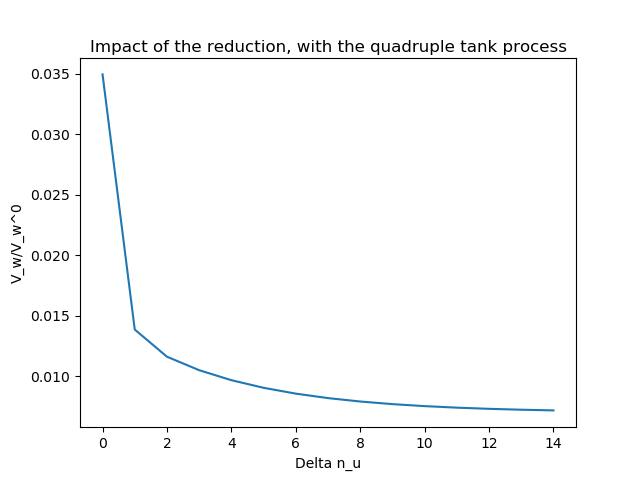
\includegraphics[width=0.9\linewidth]{lin_sys_reduction_seq_control_len}
  \caption{Impact of the variable $\Ninputs$ over the size of the possible state of the reduced system. It does not worth to take $\Ninputs$ greater than 1 since the boundaries of the reduce system does not decrease that much and the complexity of the model exponentially dependant of the number of controls.}
  \label{reduced_system_bounds}
\end{figure}

The next table summaries the gains and loses of this reduction on the previously established criteria.

\begin{tabular}{ l|ll }
& Initial model & Reduced model\\ \hline
Nodes & $\prod_{i=1}^n N_i$ & $\left | U \right |^{\Ninputs} \prod_{i=1}^{n_c} N_i $\\ 
$|U|$ & $n_u$ & $n_u$\\
$V_w$ &  & bigger \\
\end{tabular}

\subsection{Size of the reached sets}
Talk about the continuous model

Studying the continuous case can give us a good insight about the influence of the sampling rate over the size of the estimated sets.

For the following model:
\begin{equation}
\dot{\x} = A \x + B \vu + E \w
\end{equation}
we can show that for a quadratic Lyapunov function, we can compute an upper bound on the size of the successors of the model.
The noise is moving the state from its equilibrium position, and every increase of the noise magnitude increase the number of successors.

The figure \ref{fig:lyap_deacr} is a plot of the lyapunov decrease.
From this graphic we can see that as the time passes, the number of successors between the reduced and the non reduced abstraction tend to be the same. This mean that when the sampling rate is slower than the dynamics, the number of successors of the models will almost the same (compared to the volume of successors).
However, when the sampling rate is faster than the dynamic, the reduction over approximate the set of successors, and it might be more interesting to keep the observation of the model.

Ones should note as well than the number of successors is always smaller for the abstraction than for the reduced model. This come from the fact that the set of all the possible estimation of the state must contain the measure.
However, when it comes to state space discretization this difference might not be the same as the knowledge of the sequence of past inputs is not used. 

\subsection{Reachability/Controllability}
Reachable sets are computed with the invariant set. As the invariant set is an over approximation of the state, it is always possible to find a discretization of the unobserved subspace that create less successors than the estimation of the state.
This might results in an abstraction that is unusable whatever the number of memories we are using or the sampling rate of the model.

\subsection{Notes}
Self loops are not desirable.

Self loops hide any time information (that is why I have been working on the time information chapter).

In the case of the reduction of the abstraction.